\chapter{Model and methods}
\label{chap:modmet}
To produce results for the thesis, a formulation of the Weather Research and Forecasting (WRF) Model called the Advanced Research WRF (ARW) has been used. The model is described in the first part of this chapter. Then follows a description of the model setup and the different physics schemes that were chosen for this study, before a summary of the different runs that were performed. Ending the chapter are two short sections on the input data and processing of the model output.
%---------------------
\section{Description of the WRF-ARW Modeling System}
\label{sec:modeldes}
%---------------------
The version of the WRF-ARW modeling system used is 3.6.1, which was released in April 2014. The model is primarily developed at the National Centre for Atmospheric Research (NCAR) in Boulder, Colorado. The ARW model is the first fully compressible conservative form nonhydrostatic model designed for both research and operational numerical weather prediction (NWP) applications~\citep{Skamarock2008}. 

As can be seen from figure~\ref{fig:wrfflowchart} the WRF-ARW Modeling System consists of four major programs~\citep{Wang2015}:
\begin{itemize}
\item The WRF Prepocessing System (WPS)
\item WRF-Data Assimilation (WRF-DA)
\item ARW solver
\item Post-processing \& Visualization tools
\end{itemize}

\begin{figure}
\centering
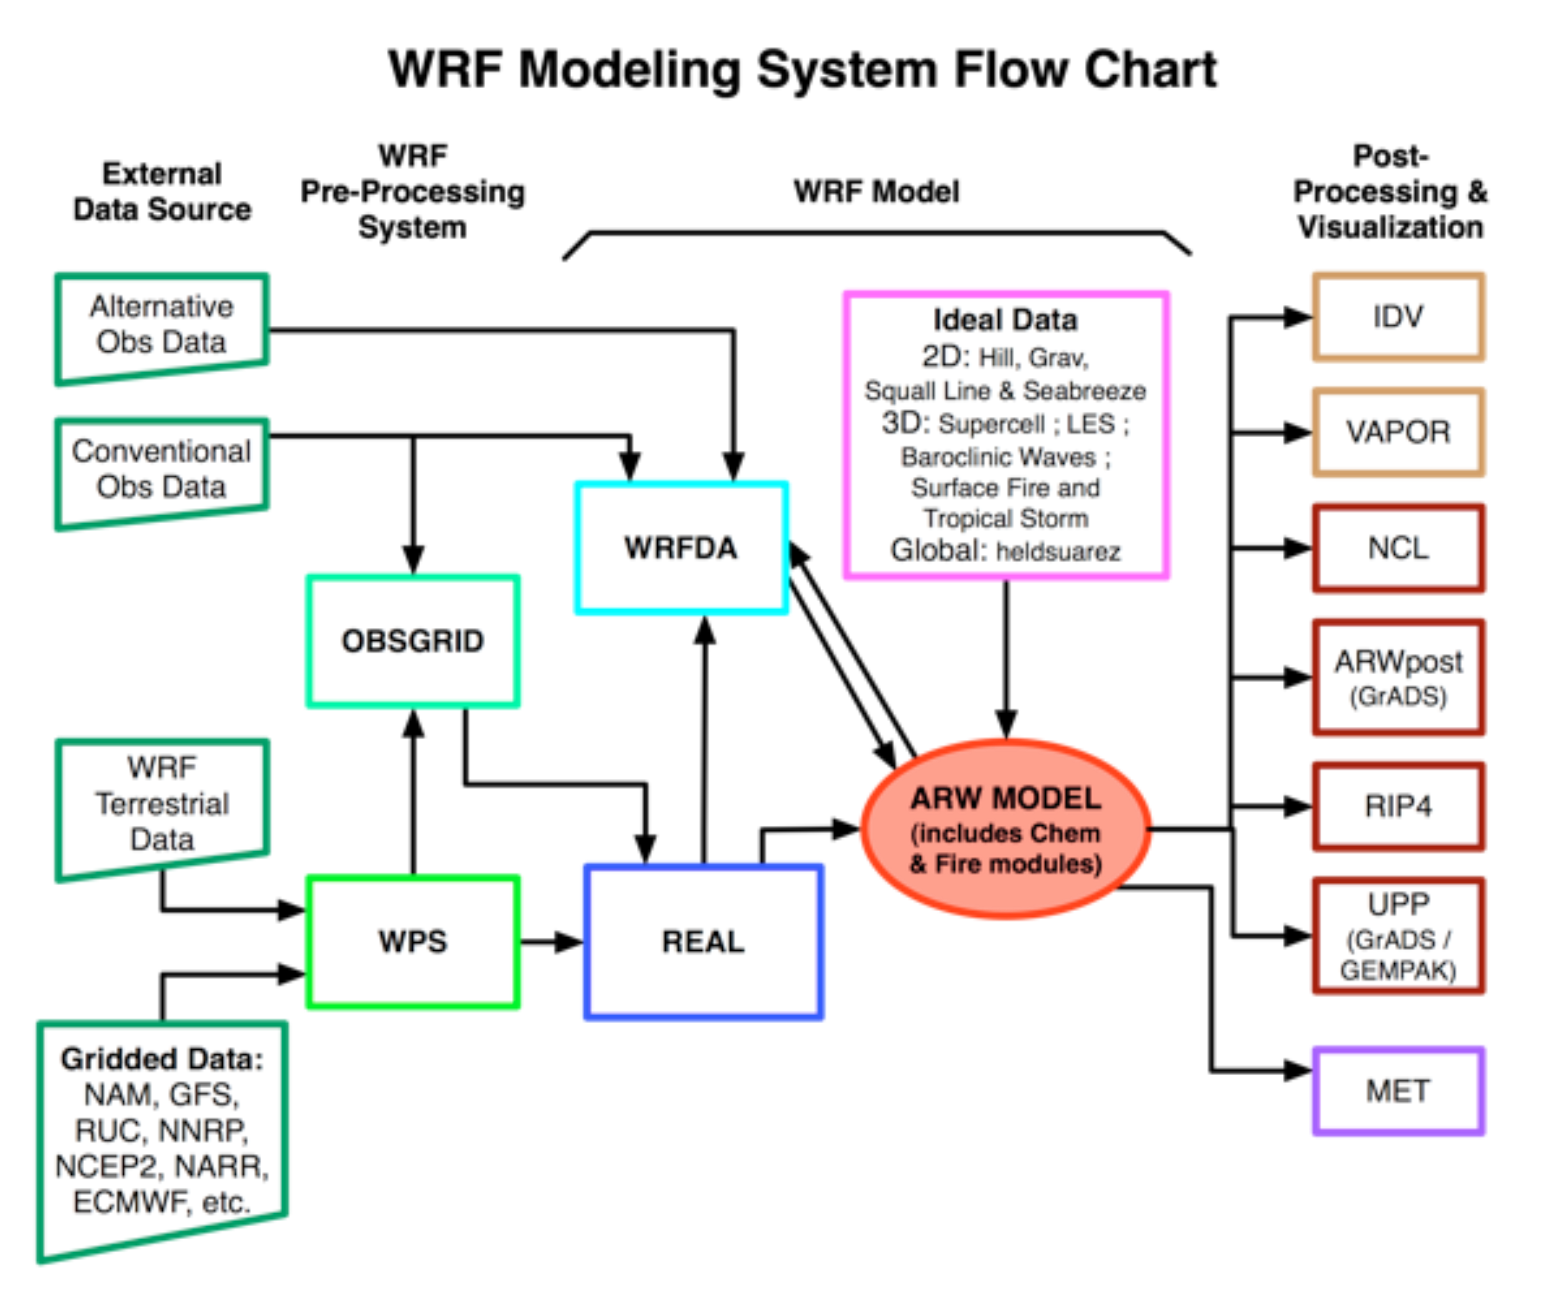
\includegraphics[width=0.9\textwidth]{model_methods/wrfflowchart}
\caption{Flowchart for the WRF ARW Modeling System Version 3. From~\citet{Wang2015}.}
\label{fig:wrfflowchart}
\end{figure}

WPS is used primarily for real data simulations~\citep{Wang2015}, like the study presented in this thesis. A real-data simulation means that it has been initialized by observations and reanalysis, not artificial data. WPS' functions include defining simulation domains, interpolating terrestrial data and degribbing and interpolating meteorological data from another model to this simulation domain~\citep{Wang2015}. WRF-DA is optional and can be used to ingest observations into the interpolated analyses created by WPS~\citep{Wang2015}, but was not used in this study. The ARW solver is the key component of the modeling system, which is composed of several initialization programs for idealized, and real-data simulations, and the numerical integration program~\citep{Wang2015}.% Fully compressible nonhydrostatic equations with hydrostatic options, regional and global applications, complete coriolis and curvature terms and that vertical grid-spacing can vary with height are among the WRF models key features according to~\citet{Wang2015}.

\subsection{The vertical coordinate}
The continuous equations solved in the ARW model are the Euler equations cast in a flux form where the vertical coordinate, $\eta$, is defined by a normalized hydrostatic pressure,
\begin{equation}
\eta = (p_h - p_{ht})/\mu 
\end{equation}
where $\mu = (p_{hs} - p_{ht})$~\citep{Skamarock2008}. $p_h$ is the hydrostatic component of the pressure and $p_{hs}$ and $p_{ht}$ are the values of the hydrostatic pressure in a dry atmosphere at the surface and top boundaries respectively~\citep{Skamarock2008}.

The vertical coordinate is the traditional $\sigma$ coordinate used in many hydrostatic atmospheric models, shown in figure~\ref{fig:sigma}.
\begin{figure}[h]
\centering
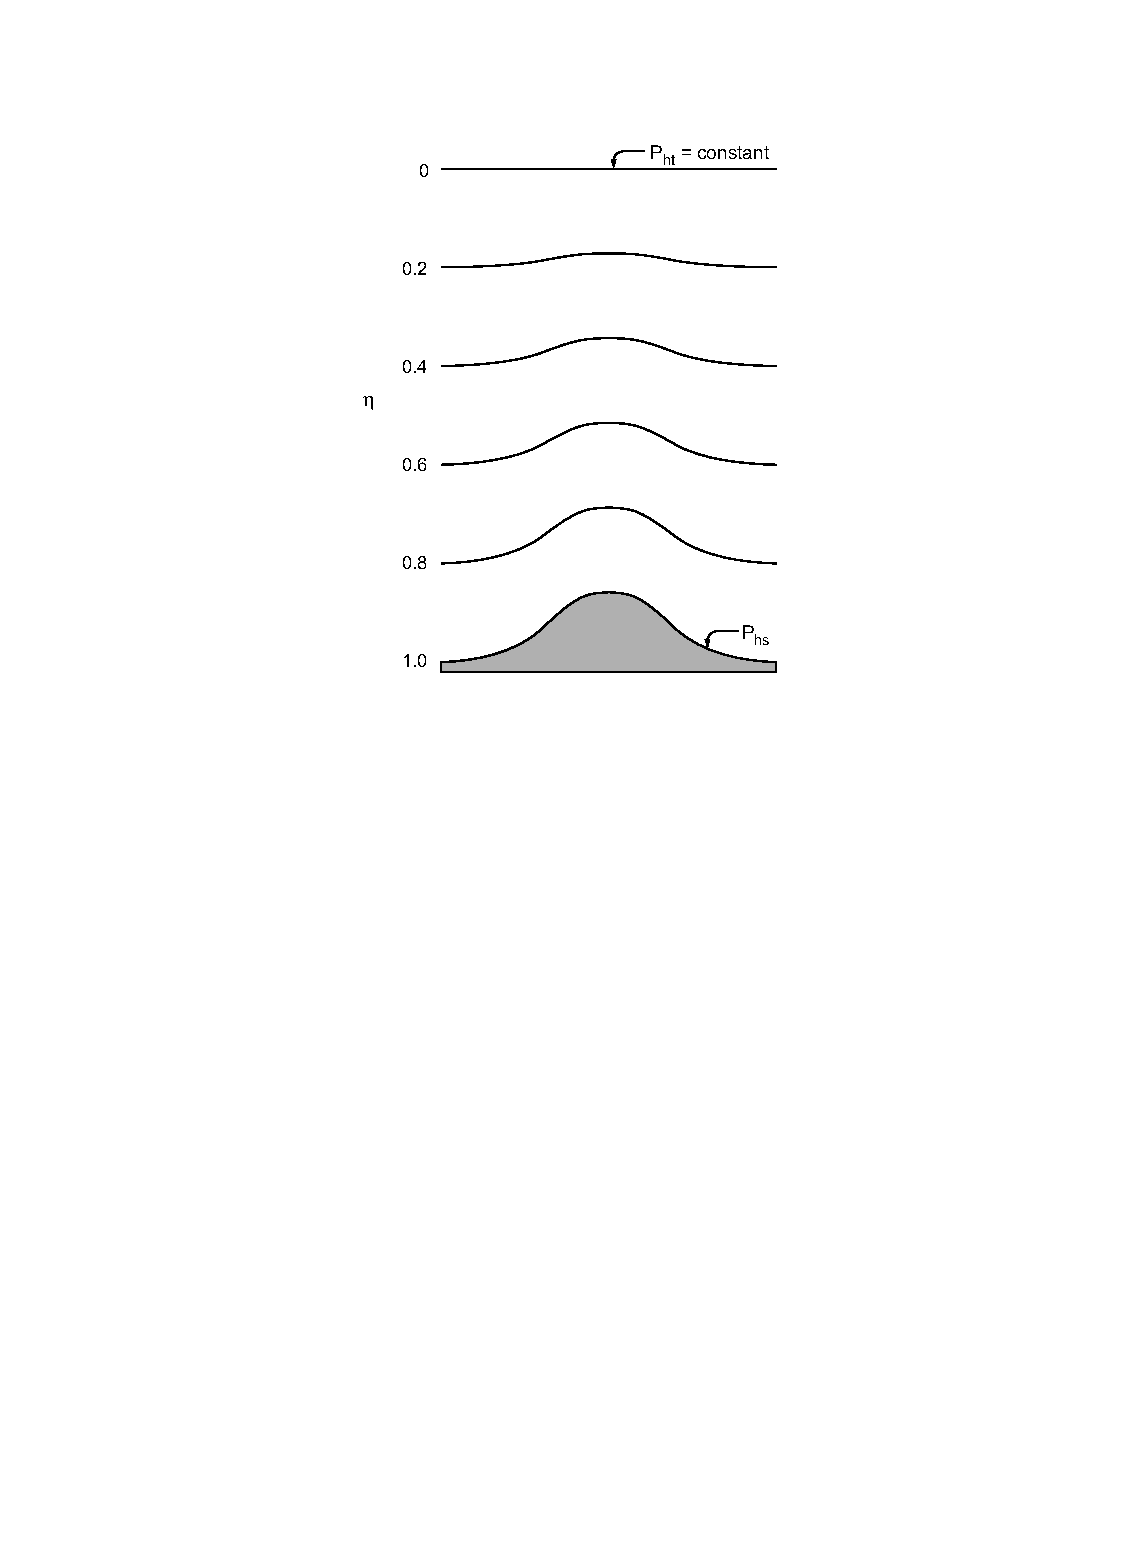
\includegraphics[scale=0.9]{model_methods/sigma.pdf}
\caption{This figure is shown as presented in~\citet{Skamarock2008}, and is a schematic of the terrain following a $\sigma$ coordinate. $P_{hs}$ and $P_{ht}$ are the hydrostatic pressure at the surface and top respectively.}
\label{fig:sigma}
\end{figure}



%--------- Stuff on staggered grid.
\subsection{Staggered grid}
The WRF-model uses a staggered grid, which means that some variables lie in the middle of a gird box, and other on the sides of the box. The pressure for example is in the middle of the grid box, and the winds on each side of the box use the pressure in the middle of one box, and the middle of the box next to it as reference for calculating the winds at the grid box sides. A staggered grid saves computational time since the a variable at point a needs only the values at a+1/2, and a-1/2, in stead of a+1 and a-1, which is more computationally costly.

The staggered grid therefore reduces the computation time of the WRF-ARW modeling system.

This is important to know, also for the variables in the vertical. If a cloud effective radius, $r_e$, for example lies between two levels, in the middle of a layer, or if they have values exactly on the levels.

Figure~\ref{fig:stagger} shows the staggered C-grid used in the WRF-model. The C-grid is the most used staggered grid in nonhydrostatic NWP and research models~\citep{Skamarock2008}.

\begin{figure}%[h]
\centering
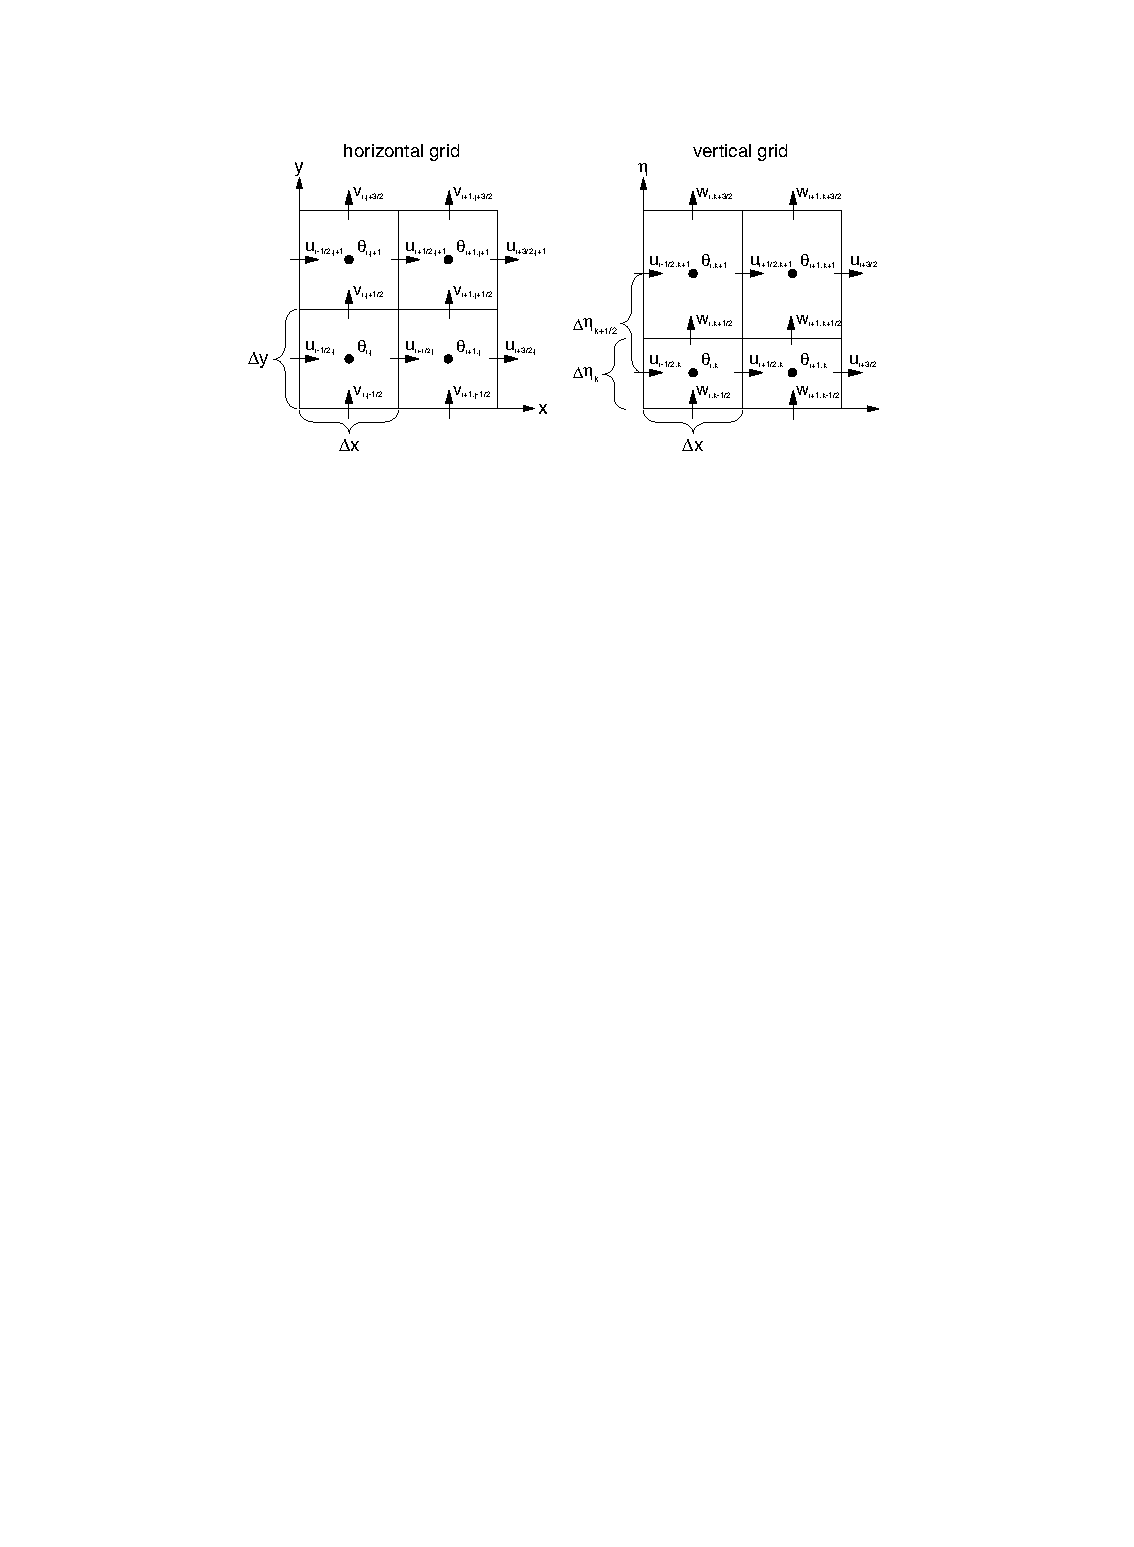
\includegraphics[width=\textwidth]{model_methods/gridstagger.pdf}
\caption{This figure is shown as presented in~\citet{Skamarock2008}, and shows the staggering for the C-grid. The horizontal staggering to the left, and the vertical staggering to the right.}
\label{fig:stagger}
\end{figure}

The selection of physics schemes in WRF-ARW are numerous. The choice of schemes treating microphysics in clouds and aerosols, and the radiation are presented in the following section about the model setup.
%---------------------
\section{Model setup}
\label{sec:modelsetup}
%---------------------
The model was ran with a 4~km$\times$4~km horizontal grid point spacing, with 300$\times$300 grid points, and 72 vertical layers, with the model top at 10~hPa.
The area covers parts of the Beaufort Sea, by Canada and Alaska. This area was chosen because data from the area has been used for related studies~\citep{Intrieri2002,Shupe2004,Kay2009,Wu2012,Palm2010,Schweiger2008} %sjekk dette!!,
as mentioned in Chapter~\ref{chap:introduction} and described in Chapter~\ref{chap:background}.%, to give the reader some background material and an understanding of the subject of this study.
The area is not completely ice free any part of the year,% @cite,
 and provides a good place to simulate cloud-sea ice interaction. The area is over several time zones but is approximately 7 hours behind UTC time. The times given in the WRF-ARW modeling system are UTC. The model was ran for a period of 5~days, 1st to 6th of September 2012. This is approximately when the record low ice extent in the Arctic was set (eg. National Snow and Ice Data Centre, U.S.A.,~\citet{Beitler2012}).

The vertical layers in the ARW model are often referred to as eta levels, because of the choice of $\eta$ as the vertical coordinate. These levels have uneven vertical spacing. The fact that this $\eta$ is the traditional $\sigma$-coordinate, means that the altitude of each level is dependent on pressure, therefore the level height varies in both time and space. As a consequence of pressure dependence, the levels in the lower troposphere are closer to each other than the levels higher up in the troposphere. Therefore the low clouds in the area can be resolved. Approximate heights for the lowest 11 eta levels is shown in Table~\ref{tab:etaheights}.

\begin{table}[H]
\centering
\caption{Approximate height for each level in meters above the surface.}
\label{tab:etaheights} 
\begin{tabular}{C{4.cm} C{5.cm}}
\centering
\textbf{Eta level} & \textbf{Approximate height}\\ \hline
1 & 10~m\\
2 & 50~m\\
3 & 130~m\\
4 & 230~m\\
5 & 370~m\\
6 & 530~m\\
7 & 650~m\\
8 & 950~m\\
9 & 1250~m\\
10 & 1400~m\\
11 & 1600~m
\end{tabular}
\end{table}

%The sea ice in the area was removed, to get results from comparing output from the model runs without ice, to those with ice.


%Choice of schemes and reasons should be presented. As should how WPS and real.exe and wrf.exe works. At least short about what they do and contribute with to get to the end results. Explain some of the improvements in the micro physics scheme in combination with the revised radiation schemes (RRTMG for SW and LW).
\subsection{Choices of physics in the model}
%Based on the WRF-ARW Version 3 User's Guide by~\citet{Wang2015}.
%Based on the description of ARW Version 3 from \citet{Skamarock2008a}. 
The physics options in WRF fall into several categories, each containing several choices. Table~\ref{tab:physics} shows some of the different categories and the choice of scheme, for this study, within each of those categories.

\begin{table}[H]
\centering
\caption{Table of physics categories and choice of scheme for this thesis}
\label{tab:physics} 
\begin{tabular}{L{4cm} L{7cm}}
\centering
\textbf{Physics categories} & \textbf{Scheme selected within category}\\ \hline
(1) microphysics & aerorol-aware ~\citep{Reisner1998, Thompson2004, Thompson2008, Thompson2014}. Option 28.\\
(2) cumulus parameterization & Grell 3D  @cite authors. Option 5.\\
(3) planetary boundary layer (PBL) &  Yonsei University scheme @cite authors. Option 1.\\
(4) land-surface model & Noah Land Surface Model @cite authors. Option 2.\\
(5) radiation & RRTMG LW \& SW ~\citep{Mlawer1997, Iacono2000, Iacono2003, Iacono2008}. Radiation options 4.
\end{tabular}
\end{table}

The ARW model offers a wide selection of schemes to treat different physics that one wants represented in the model. The schemes treat the physics slightly differently and some schemes are better for certain horisontal and vertical resolutions than others, so one needs to be careful when choosing how the model is to treat the physics. For my thesis, the especially relevant scheme to mention is the cloud microphysics scheme that I chose, which is the aerosol-aware scheme described in~\citet{Thompson2014}. When studying cloud and rediation response to removal of sea ice we might expect an increase in aerosols from the open ocean and increased sea traffic. The aerosols are therefore also relevant for the choice of schemes, and the aerosol-aware scheme includes the necessary processes for this study.

%The choice of cumulus parameterization was based on the grid resolution, and the best fit for it. A horisontal grid point spacing of 4~km can be fine enough to not use cumulus parameterization, but in this thesis we chose a parameterization that was more suitable for grid point spacings less than 10~km, the Grell 3D parameterization. Grell 3D is an improved multi-closure, multi-parameter ensamble method with typically 144 sub-grid members, that may be used on high resolution~\citep{Wang2015}, like my 4~km grid point spacing.
%---------
%Yonsei University scheme was chosen for the PBL. It is a non-local-K scheme with explicit entrainment layer and parabolic profile in unstable mixed layer~\citep{Wang2015}.
%---------
%The land-surface model choice came to Noah Land Surface Model. The Noah Land Surface Model, is a unified NCEP/NCAR/AFWA (National Centers for Environmental Prediction, National Centre for Atmospheric Research, Air Force Weather Agency) scheme with soil temperature and moisture in four layers which provides sensible and latent heat fluxes to the PBL scheme~\citep{Wang2015}. Additionally, it predicts soil ice, and fractional snow cover effects, which could be important in the Arctic, but it is probably not the most important choice, since there is very little land in the area investigated, see figure~\ref{fig:area} in Chapter~\ref{chap:introduction}.
%----------
%The radiation schemes were chosen simply because they are the best match for the microphysics scheme at the time of writing. According to~\citet{Thompson2014} the Rapid Radiative Transfer Model (RRTM) for General Circulation Models (GCMs) (RRTMG) schemes for SW and LW are the only radiation schemes which include the effects of the effective radii calculated in aerosol-aware. The RRTMG schemes are accurate schemes using look-up tables for efficiency, and accounts for multiple bands and microphysics species, and includes the Monte Carlo Independent Column Approximation (MCICA) method of random cloud overlap~\citep{Wang2015}.

\subsubsection{The aerosol-aware scheme}
The microphysics includes explicitly resolved water vapor, cloud, and precipitation processes. The aerosol-aware scheme was chosen so that the study would have scavenging of aerosols included and have proper enough representation of aerosols to study aerosol-cloud interactions, without using the WRF model coupled with chemistry (WRF-Chem).
According to the ARW User's Guide by~\citet{Wang2015}, the aerosol-aware scheme considers water- and ice-friendly aerosols, and a climatological dataset may be used to specify initial and boundary conditions for the aerosol variables. I have used this climatological dataset, which is explained in Section~\ref{sec:inputdata}~Input~data. The scheme uses a monthly mean for aerosol number concentrations derived from multi-year (2001-2007) global model simulations in which particles and their precursors are emitted by natural and anthropogenic sources and are explicitly modeled with multiple size bins for multiple species of aerosols by the Goddard Chemistry Aerosol Radiation and Transport (GOCART) model %(@desiterteGinoux2001)
~\citep{Thompson2014}.
The aerosol-aware scheme~\citep{Thompson2014} is built on the schematic shown in figure~\ref{fig:microphysics}, from~\citet{Reisner1998}. It is a double moment scheme, which means it computes both mass mixing ratios, Q, and number concentrations, N, for the same water species (hydrometeors). 

\begin{figure}[h]
\centering
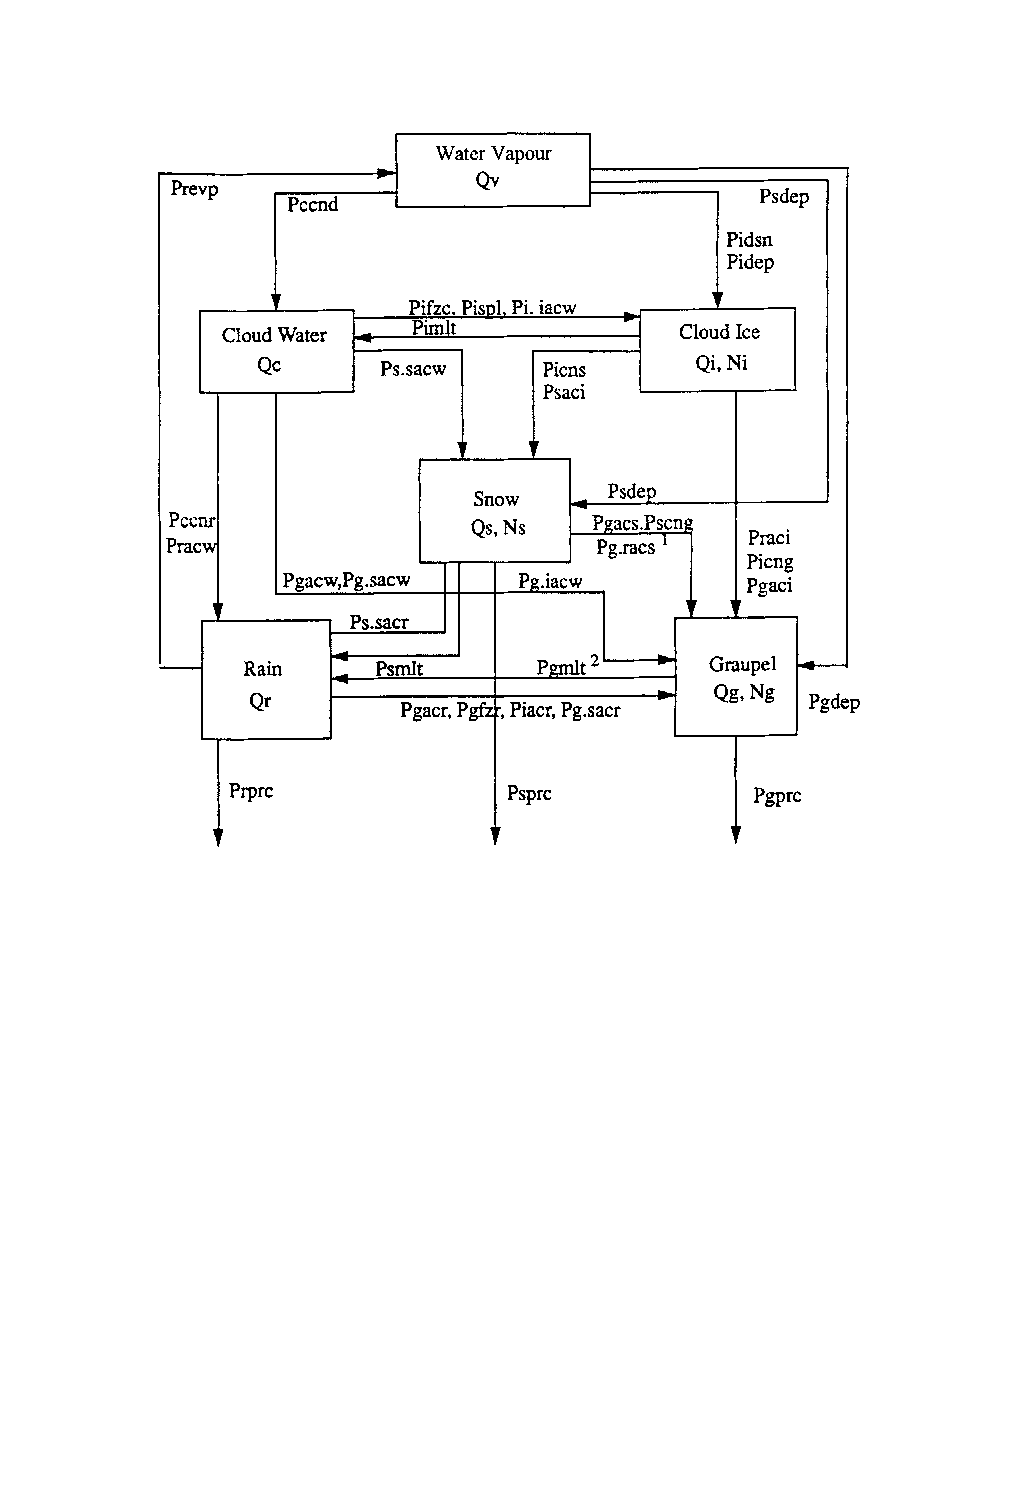
\includegraphics[width=0.9\textwidth]{model_methods/microphysics.pdf}
\caption{Cloud microphysical parameterization scheme typically used i NWP models as shown in~\citet{Reisner1998}. A full list of the acronyms used in the schematic can be found in~\citet{Reisner1998}.}
\label{fig:microphysics}
\end{figure}

Figure~\ref{fig:microphysics} show the processes in the microphysics scheme developed by~\citet{Reisner1998}, which the first bulk microphysics scheme by Thompson~\citep{Thompson2004} was based on. The aerosol-aware scheme~\citep{Thompson2014} is an extension of the updated Thompson bulk microphysics scheme described in~\citet{Thompson2008}. The figure shows a schematic of five hydrometeors, cloud water (c), rain (r), ice (i), snow (s) and graupel (g), and if just the mass mixing ratio is calculated or if both the mass mixing ratio and the number concentration is calculated. For each of the hydrometeors, prognostic equations are used with all the sources and sink terms included.%, as exemplified by this equation from~\citet{Reisner1998}?
 % which was originally built on this~\citep{Thompson2004}, but there is not much left of it in the code now (@cite the code comments?).
 
\subsubsection{The RRTMG radiation schemes}
According to~\citet{Thompson2014} the Rapid Radiative Transfer Model (RRTM) for General Circulation Models (GCMs) (RRTMG) schemes for SW and LW~\citep{Mlawer1997, Iacono2000, Iacono2003, Iacono2008} are the only radiation schemes which include the effects of the effective radii calculated in aerosol-aware. These were therefore used in combination with the aerosol-aware cloud microphysics scheme. The RRTMG schemes are accurate schemes using look-up tables for efficiency, and accounts for multiple bands and microphysics species, and includes the Monte Carlo Independent Column Approximation (MCICA) method of random cloud overlap~\citep{Wang2015}.
%The RRTM scheme described in~\citet{Mlawer1997} uses the correlated-k method, which is an appriximated technique for the accelerated calculation of fluxes and cooling rates for inhomogeneous atmospheres~\citep{Mlawer1997}. %\textbf{@define inhomogeneous atmosphere}.
%The correlated-k method is capable of achieving accuracy comparable with that of line-by-line models with an extreme reduction in the number of radiative transfer operations performed~\citep{Mlawer1997}, which by that reduces computational cost and increases computational efficiency. The Line-By-Line Radiative Transfer Model (LBLRTM) is used both to calculate the absorption coefficients used to generate the k distributions needed by RRTM and  to evaluate the RRTM calculations of fluxes and cooling rates~\citep{Iacono2000}. 

\section{Model runs}
The results presented in the next chapter are based on six different runs. The control run is the run where the aerosol climatological dataset has been used unchanged, and where the sea ice is kept as it was in the downloaded input data, see Section~\ref{sec:inputdata}. The control run is used as a base to compare the other runs to, those with no ice and/or increased aerosol number concentrations.

There are three runs where the sea ice was removed, NoIce, Aero10NoIce and Aero100NoIce. The point of this is to compare the run with no ice to the control run, and see if there are any changes in the cloud properties, and SW and LW fluxes. For two of those runs the aerosol number concentration was also increased, these can be compared with the control run, and the other runs that have ice, but the same aerosol number concentrations.

The number of water- and ice-friendly aerosols were multiplied by 10 and 100 both with and without sea ice for 4 runs in total: Aero10 and Aero100 with ice, and as mentioned above, Aero10NoIce and Aero100NoIce without ice. The goal is to find changes in cloud properties, and radiation fluxes compared to those in the control run.

Table~\ref{tab:runs} shows an overview of the different runs that have been executed, whose output have been used for production of figures presented in the next chapter.
%\begin{table}[H]
%\centering
%\caption{Table showing the name of the runs and what is included}
%\label{tab:runs} 
%\begin{tabular}{L{2.3cm} L{2.3cm} L{2cm} L{1.5cm} L{1cm} L{1cm} L{3cm}}
%\centering
%Name & Horisontal resolution & Dimensions & Vertical layers & $\Delta$t & Sea ice & Aerosol concentration\\ \hline
%control & 4~km x 4~km & 300 x 300 & 72& 24~s & yes & control\\
%NoIce & 4~km x 4~km & 300 x 300 & 72 & 24~s & no & control\\
%Aero10 & 4~km x 4~km & 300 x 300 & 72 & 24~s & yes & control x 10\\
%Aero10NoIce & 4~km x 4~km & 300 x 300 & 72 & 24~s & no & control x 10\\
%Aero100 & 4~km x 4~km & 300 x 300 & 72 & 24~s & yes & control x 100\\
%Aero100NoIce & 4~km x 4~km & 300 x 300 & 72 & 24~s & no & control x 100 \\
%\end{tabular}
%\end{table}
%
%Which table?
\begin{table}[H]
\centering
\caption{Table showing the names of the runs and if they have sea ice or not, and if the aerosol concentration has been increased by a factor of 10 or 100 through input files. All the runs have the same horisontal resolution of 4~km$\times$4~km, dimensons 300$\times$300, 72 vertical layers and time step 24 s.}
\label{tab:runs} 
\begin{tabular}{L{2.3cm} L{2cm} L{3cm}}
\centering
Name & Sea ice & Aerosol concentration\\ \hline
control & initial & climatology\\
NoIce & removed & climatology\\
Aero10 & initial & climatology$\times$10\\
Aero10NoIce & removed & climatology$\times$10\\
Aero100 & initial & climatology$\times$100\\
Aero100NoIce & removed & climatology$\times$100\\
\end{tabular}
\end{table}


\subsection{Manipulation of input files}
The input files for the ARW solver, created by WPS and REAL (see figure~\ref{fig:wrfflowchart}) were manipulated by use of the NetCDF Operator (NCO) tool ncap2. In these files the sea ice was removed for the runs without sea ice (NoIce, Aero10NoIce, Aero100NoIce) and the aerosol number concentration from the climatological dataset was multiplyed by 10 and 100 for the runs with increased aerosol concentrations by a factor of 10 and 100 respectively.
%wrfinput\_d01 and wrfbdy\_d01 are input files for domain 1, in my case the only domain, and are made by real.exe. These files are then used as initialization or forcing when wrf.exe is run.
%To run the model without ice and with an increased number of aerosols I manipulated the input files for WRF. I used a netCDF Operator (NCO) tool, ncap2. This allowed me to manipulate the netCDF files from my terminal window in the folder where they were located.
%Elaborate on removal or placing of sea ice. Elaborate on multiplying the aerosol number concentration with a factor 10 or 100. By use of ncap2 from NetCDF (NCO).

%---------------------
\section{Input data}
\label{sec:inputdata}
%---------------------
The model runs were initialized with data downloaded from the European Centre for Medium-Range Weather Forecasts (ECMWF)%~\citet{ecmwf}
%@cite web page.%was downloaded from their site and used as input for initial and boundary?? conditions.
The downloaded data is from the ERA-Interim dataset, which is a global atmospheric reanalysis from 1979 to present and continues to be updated in real time%~\citet{ecmwf}.%@make bib for ecmwf
Through WPS the data from ERA-Interim was interpolated over the area, with a 2 degree minute spacing between the points, to be used to initialize the model. The data used is in 6-hourly atmospheric fields on pressure levels, for the first five days of September 2012, which was the period the model was run for. This is done to make sure the initial meteorological conditions are the same in every run, so that the effects of changing a variable in the input files for the modeling system are only due to that change.

To use the climatological aerosol dataset, the file containing monthly means had to be called through WPS. The aerosol input data includes mass mixing ratios of sulfates, sea salts, organic carbon, dust, and black carbon from a 7-yr simulation with 0.5$^{\text{o}}$ longitude by 1.25$^{\text{o}}$ latitude spacing~\citep{Thompson2014}.

%---------------------
\section{Processing of the results}
%---------------------
Figures presented in my thesis, I made (unless other is stated) by use of NCL (National Centre for Atmospheric Research (NCAR) Command Language) and/or MatLab. For the NCL scripts I found a lot of help and inspiration from the example scripts for WRF-users available at (URL for examples).

%I made all the figures that are over maps with NCL, the others were made with MatLab provided by the University of Oslo.

%MathWorks, it is very useful and easy to use.

%NCL it is free and there are a lot of available example scripts to quickly learn how to use the graphics.